\documentclass[12pt,aspectratio=169]{beamer}

\usepackage{minted}

\usetheme[progressbar=frametitle, numbering=fraction]{metropolis}
\usepackage{appendixnumberbeamer}

\usepackage{booktabs}
\usepackage[scale=2]{ccicons}

\usepackage{pgfplots}
\usepgfplotslibrary{dateplot}

\usepackage{xspace}
\usepackage{tikz}
\newcommand{\themename}{\textbf{\textsc{metropolis}}\xspace}

% Chinese Fonts (Fontset: fandol,ubuntu)
\usepackage{ctex}

% Math Fonts
\usefonttheme{professionalfonts} 
\usepackage{mathspec}
% \setsansfont[BoldFont={Fira Sans},Numbers={OldStyle}]{Fira Sans Light}
% \setmathsfont(Digits)[Numbers={Lining, Proportional}]{Fira Sans Light}

% Change Color of the theme
\usepackage{xcolor}
\definecolor{DarkGrey}{HTML}{353535}
\definecolor{ECNURed}{RGB}{164,31,53}
\definecolor{ECNUBrown}{RGB}{134,117,77}
\setbeamercolor{normal text}{ fg= DarkGrey  }
\setbeamercolor{alerted text}{ fg= ECNURed  }
\setbeamercolor{example text}{ fg= ECNUBrown  }

% Bolder Fonts for presenting in a large room 
\setsansfont[BoldFont={Fira Sans SemiBold}]{Fira Sans Book}

\title{组合数学算法与应用}
\subtitle{二项式系数、斐波那契数、卡特兰数与斯特林数}
\date{\today}
\author{罗江楠}
\institute{哈尔滨工业大学(威海)}
\titlegraphic{\hfill
\includegraphics[height=1cm]{hitwh.png}}

\begin{document}

\maketitle

\begin{frame}{目录}
  \setbeamertemplate{section in toc}[sections numbered]
  \tableofcontents[hideallsubsections]
\end{frame}

\section[引言]{Introduction}

\begin{frame}[fragile]{引言}
  \begin{itemize}
    \item 组合数学在 ACM 中多为数数题出现
    \item 结果一般较大,通常采用对某数取模的方法来简化计算,注意欧拉定理和扩展欧拉定理的使用
    \item 如果推不出式子,可以考虑先使用动态规划、暴力等方法求出一小范围内的解去观察规律
  \end{itemize}
\end{frame}

\section[二项式系数]{Binomial Coefficient}

\subsection[二项式系数]{Definition}

\begin{frame}[fragile]{二项式系数}
$(1+x)^n$ 的多项式展开式中 $x^k$ 项的系数定义为二项式系数,记为 ${n \choose k}$。

也可以用来表示从 $n$ 个物品中取出 $k$ 个物品的方案数量,也可记为 $C_n^k$。

$$
C_n^k = {n \choose k} = \frac{n!}{k!(n-k)!}
$$
\end{frame}

\begin{frame}[fragile]{二项式系数}
一堆可能用的上的等式

$$
{n \choose m} = {n-1 \choose m} + {n-1 \choose m-1}
$$

$$
{n \choose m} = \frac{n}{m} {n-1 \choose m-1}
$$

$$
\sum_{i=0}^{n} {i \choose m} = {n+1 \choose m+1}
$$

$$
{n \choose r}{r \choose k} = {n \choose k} {n-k \choose r-k} = {n \choose k} {n-k \choose n-r}
$$
\end{frame}

\subsection[例题:序列统计]{Example: Sequence Statistics}

\begin{frame}[fragile]{例题:序列统计}
求长度在 $1$ 到 $N$ 之间,并且每个元素大小都在 $[L, R]$ 区间内的单调不降序列的数量,结果对素数 $p=10^6+3$ 取模。

$1 \le N \le 10^9, 1 \le L \le R \le 10^9, T \le 100$
\end{frame}

\begin{frame}[fragile]{例题:序列统计}
不妨设 $M=R-L+1$。

首先考虑长度为 $n$ 的满足条件的序列的数量。

由于要求序列不降,因此答案只与每种不同取值的数量有关。

问题转化成 $n$ 个球放到 $M$ 个盒子里的经典问题。

因此当长度为 $n$ 时序列的数量即为 ${n+M-1 \choose M-1}$
\end{frame}

\begin{frame}[fragile]{例题:序列统计}
最终结果即为

$$
\begin{aligned}
\sum_{n=1}^{N} {n+M-1 \choose M-1} \pause
&= \sum_{n=M}^{N+M-1} {n \choose M-1} \\ \pause
&= \sum_{n=0}^{N+M-1} {n \choose M-1} - {M-1 \choose M-1} \\ \pause
&= {N+M \choose M} - 1
\end{aligned}
$$
\end{frame}

\subsection[卢卡斯定理]{Lucas Theorem}

\begin{frame}[fragile]{卢卡斯定理}
当 $p$ 为素数时

$$
{n \choose m} = {\left\lfloor n/p \right\rfloor \choose \left\lfloor m/p \right\rfloor} {n \mod p \choose m \mod p} \pmod{p}
$$
\end{frame}

\subsection[二项式定理]{Binomial Theorem}

\begin{frame}[fragile]{二项式定理}
二项式定理

$$
(a+b)^n = \sum_{i=0}^{n} {n \choose i} a^{n-i} b^{i}
$$
\end{frame}

\begin{frame}[fragile]{二项式定理}
当 $a=1, b=1$ 时有

$$
\sum_{i=0}^{n} {n \choose i} = 2^n
$$

当 $a=1, b=-1$ 时有

$$
\sum_{i=0}^{n} (-1)^i {n \choose i} = [n = 0]
$$
\end{frame}

\subsection[二项式反演]{Binomial Transform}

\begin{frame}[fragile]{二项式反演}
形式一

$$
f(n) = \sum_{i=0}^{n} (-1)^i {n \choose i} g(i)
\quad \Longleftrightarrow \quad
g(n) = \sum_{i=0}^{n} (-1)^i {n \choose i} f(i)
$$
\end{frame}

\begin{frame}[fragile]{二项式反演:证明}
若要证明原命题成立,即证

$$
\begin{aligned}
  f(n) &= \sum_{i=0}^{n} (-1)^i {n \choose i} g(i) \\
       &= \sum_{i=0}^{n} (-1)^i {n \choose i} \sum_{j=0}^{i} (-1)^j {i \choose j} f(j) \\ \pause
       &= \sum_{i=0}^{n} \sum_{j=0}^{i} (-1)^{i+j} {n \choose i} {i \choose j} f(j) \\ \pause
       &= \sum_{j=0}^{n} \sum_{i=j}^{n} (-1)^{i+j} {n \choose j} {n - j \choose n - i} f(j)
\end{aligned}
$$
\end{frame}

\begin{frame}[fragile]{二项式反演:证明}
$$
\begin{aligned}
  f(n) &= \sum_{j=0}^{n} \sum_{i=j}^{n} (-1)^{i+j} {n \choose j} {n - j \choose n - i} f(j) \\
       &= \sum_{j=0}^{n} {n \choose j} f(j) \sum_{i=j}^{n} (-1)^{i+j} {n - j \choose n - i} \\ \pause
       &= \sum_{j=0}^{n} {n \choose j} f(j) \sum_{i=0}^{n-j} (-1)^{i} {n - j \choose i} \\ \pause
       &= \sum_{j=0}^{n} {n \choose j} f(j) [n = j] \pause = f(n)
\end{aligned}
$$

因此原命题成立。
\end{frame}

\begin{frame}[fragile]{二项式反演}
形式一

$$
f(n) = \sum_{i=0}^{n} (-1)^i {n \choose i} g(i)
\quad \Longleftrightarrow \quad
g(n) = \sum_{i=0}^{n} (-1)^i {n \choose i} f(i)
$$

形式二

$$
f(n) = \sum_{i=0}^{n} {n \choose i} g(i)
\quad \Longleftrightarrow \quad
g(n) = \sum_{i=0}^{n} (-1)^{n-i} {n \choose i} f(i)
$$
\end{frame}

\begin{frame}[fragile]{二项式反演}
形式三

$$
f(n) = \sum_{i=n}^{m} (-1)^i {i \choose n} g(i)
\quad \Longleftrightarrow \quad
g(n) = \sum_{i=n}^{m} (-1)^i {i \choose n} f(i)
$$

形式四

$$
f(n) = \sum_{i=n}^{m} {i \choose n} g(i)
\quad \Longleftrightarrow \quad
g(n) = \sum_{i=n}^{m} (-1)^{i-n} {i \choose n} f(i)
$$
\end{frame}

\subsection[例题:集合计数]{Example: Counting Sets}

\begin{frame}[fragile]{例题:集合计数}
一个有 $n$ 个元素的集合有 $2^n$ 个不同子集(包含空集),现在要在这 $2^n$ 个集合中取出若干集合(至少一个),使得它们的交集的元素个数为 $k$,求取法的方案数对 $10^9+7$ 取模后的值。

$1 \le n \le 10^6, 0 \le k \le n$
\end{frame}

\begin{frame}[fragile]{例题:集合计数}
令 $f(k)$ 为交集元素个数\textbf{刚好}为 $k$ 个时的方案数。

令 $g(k)$ 为交集元素个数\textbf{至少}为 $k$ 个时的方案数。

考虑如何计算 $g(k)$ 的值,可以先枚举选择了 $n$ 个元素中的哪 $k$ 个元素,接着在剩下的 $n-k$ 个元素构成的 $2^{n-k}$ 个子集中选取若干个来构成答案。

$$
g(k) = {n \choose k} \left(2^{2^{n-k}}-1\right)
$$
\end{frame}

\begin{frame}[fragile]{例题:集合计数}
发现会有重复计算的情况,经过分析发现每个答案被重复计算的次数与其交集元素个数有关。具体来说,满足

$$
g(k) = \sum_{i=k}^{n} {i \choose k} f(i)
$$
\end{frame}

\begin{frame}[fragile]{例题:集合计数}
利用二项式反演的形式四,可以得到

$$
\begin{aligned}
g(k) = \sum_{i=k}^{n} {i \choose k} f(i) \Longleftrightarrow
f(k) &= \sum_{i=k}^{n} (-1)^{i-k} {i \choose k} g(i) \\ \pause
f(k) &= \sum_{i=k}^{n} (-1)^{i-k} {i \choose k} {n \choose i} \left(2^{2^{n-i}}-1\right) \\ \pause
f(k) &= {n \choose k} \sum_{i=k}^{n} (-1)^{i-k} {n - k \choose n - i} \left(2^{2^{n-i}}-1\right) \\ \pause
f(k) &= {n \choose k} \sum_{i=0}^{n-k} (-1)^{i} {n - k \choose i} \left(2^{2^{n-k-i}}-1\right) \\
\end{aligned}
$$
\end{frame}

\subsection[计算方法]{Computation Method}

\begin{frame}[fragile]{二项式系数:计算方法}
利用递推式 $O(n^2)$ 预处理,之后每次 $O(1)$ 获取。

\begin{minted}{cpp}
for (int i = 0; i < n; ++ i) {
  c[i][0] = 1;
  for (int j = 1; j <= i; ++ j) {
    c[i][j] = (c[i - 1][j] + c[i - 1][j - 1]) % mod;
  }
}
\end{minted}
\end{frame}

\begin{frame}[fragile]{二项式系数:计算方法}
也可以 $O(n)$ 预处理出每个数的阶乘以及阶乘的逆元,之后每次 $O(1)$ 计算。

\begin{minted}{cpp}
for (int i = frac[0] = 1; i <= n; ++ i)
  frac[i] = ((long long) frac[i - 1] * i) % mod;
// 费马小定理求逆元
inv[n] = fast_pow(frac[n], mod - 2);
for (int i = n - 1; i >= 0; -- i)
  inv[i] = ((long long) inv[i + 1] * (i + 1)) % mod;
// 计算二项式系数
int c(int n, int m) {
  return 1ll * frac[n] * inv[m] % mod * inv[n - m] % mod;
}
\end{minted}
\end{frame}

\section[斐波那契数]{Fibonacci Numbers}

\subsection[斐波那契数]{Definition}

\begin{frame}[fragile]{斐波那契数}
斐波那契数列的定义为

$$
\begin{aligned}
F_0 &= 0 \\
F_1 &= 1 \\
F_n &= F_{n-1} + F_{n-2} \quad (n \ge 2)
\end{aligned}
$$
\end{frame}

\begin{frame}[fragile]{斐波那契数}
斐波那契数列的通项公式(Binet's Formula)

$$
F_n = \frac{1}{\sqrt{5}}\left[\left(\frac{1+\sqrt{5}}{2}\right)^n - \left(\frac{1-\sqrt{5}}{2}\right)^n\right]
$$
\end{frame}

\begin{frame}[fragile]{斐波那契数}
斐波那契数的一些特性:

$$
F_{m+n} = F_{m} F_{n-1} + F_{m+1} F_{n}
$$
\end{frame}

\begin{frame}[fragile]{斐波那契数}
简单证明:

$$
\begin{aligned}
F_{m+n} &= F_{1} F_{m+n-2} + F_{2} F_{m+n-1} \\
&= F_{1} F_{m+n-2} + F_{2} (F_{m+n-2} + F_{m+n-3}) \\
&= (F_{1} + F_{2}) F_{m+n-2} + F_{2} F_{m+n-3} \\
&= F_{2} F_{m+n-3} + F_{3} F_{m+n-2} \\
&= F_{3} F_{m+n-4} + F_{4} F_{m+n-3} \\
&= ... \\
&= F_{m} F_{n-1} + F_{m+1} F_{n}
\end{aligned}
$$
\end{frame}

\begin{frame}[fragile]{斐波那契数}
  当 $m = n$ 时有

  $$
  \begin{aligned}
  F_{2n} &= F_{n} F_{n-1} + F_{n+1} F_{n} \\
  &= F_{n} F_{n-1} + (F_{n} + F_{n-1}) F_{n} \\
  &= (2 F_{n-1} + F_{n}) F_{n} \\
  \end{aligned}
  $$

  当 $m = n-1$ 时有

  $$
  F_{2n-1} = F_{n-1}^2 + F_{n}^2
  $$
\end{frame}

\begin{frame}[fragile]{斐波那契数}
  $$
  \begin{aligned}
    F_{2n-1} &= F_{n-1}^2 + F_{n}^2 \\
    F_{2n} &= (2 F_{n-1}+  F_{n}) F_{n}
  \end{aligned}
  $$

  这两个公式经常被用于快速求解斐波那契数第 $n$ 项的值。
\end{frame}

\begin{frame}[fragile]{斐波那契数}
  一共有 $n$ 个台阶,每次可以走 $1$ 或 $2$ 个台阶,求问有多少种不同的走法。\pause

  可以简单找到递推式,发现 $f(0) = f(1) = 1, f(n) = f(n-1) + f(n-2)$,这个就是斐波那契数列的递推式。\pause

  但是换一种方式思考,我们也可以枚举总共要走多少步,然后就是一个单纯的组合数问题。\pause

  $$
  f(n) = F_{n+1} = \sum_{i=1}^{n} {i \choose n-i}
  $$
\end{frame}

\subsection[例题:undefined]{Example: Undefined}

\begin{frame}[fragile]{例题:undefined}
求

$$
\sum_{i=0}^n {n \choose i} F_{i+1}
$$

其中 $n \le 10^{10^6}$
\end{frame}

\begin{frame}[fragile]{例题:undefined}
$$
\begin{aligned}
\sum_{i=0}^n {n \choose i} F_{i+1} &= \frac{1}{\sqrt{5}} \sum_{i=0}^n {n \choose i} \left[\left(\frac{1+\sqrt{5}}{2}\right)^{i+1} - \left(\frac{1-\sqrt{5}}{2}\right)^{i+1}\right] \\ \pause
&= \frac{1}{\sqrt{5}} \left[\sum_{i=0}^n {n \choose i} \left(\frac{1+\sqrt{5}}{2}\right)^{i+1} - \sum_{i=0}^n {n \choose i} \left(\frac{1-\sqrt{5}}{2}\right)^{i+1}\right] \\ \pause
&= \frac{1}{\sqrt{5}} \left[\left(\frac{1+\sqrt{5}}{2}\right)\left(1+\frac{1+\sqrt{5}}{2}\right)^n-\left(\frac{1-\sqrt{5}}{2}\right)\left(1+\frac{1-\sqrt{5}}{2}\right)^n\right] \\ \pause
&= \frac{1}{\sqrt{5}} \left[\frac{\left(1+\sqrt{5}\right)\left(3+\sqrt{5}\right)^n}{2^{n+1}}-\frac{\left(1-\sqrt{5}\right)\left(3-\sqrt{5}\right)^n}{2^{n+1}}\right] \\
\end{aligned}
$$
\end{frame}

\begin{frame}[fragile]{例题:undefined}
观察到

$$
\begin{aligned}
\left(1+\sqrt{5}\right)^2 = 6 + 2\sqrt{5} = 2\left(3 + \sqrt{5}\right) \\
\left(1-\sqrt{5}\right)^2 = 6 - 2\sqrt{5} = 2\left(3 - \sqrt{5}\right)
\end{aligned}
$$
\end{frame}

\begin{frame}[fragile]{例题:undefined}
代入得

$$
\begin{aligned}
\sum_{i=0}^n {n \choose i} F_{i+1} &= \frac{1}{\sqrt{5}} \left[\frac{\left(1+\sqrt{5}\right)\left(\frac{\left(1+\sqrt{5}\right)^2}{2}\right)^n}{2^{n+1}}-\frac{\left(1-\sqrt{5}\right)\left(\frac{\left(1-\sqrt{5}\right)^2}{2}\right)^n}{2^{n+1}}\right] \\ \pause
&= \frac{1}{\sqrt{5}} \left[\left(\frac{1+\sqrt{5}}{2}\right)^{2n+1}-\left(\frac{1-\sqrt{5}}{2}\right)^{2n+1}\right] \\ \pause
&= F_{2n+1}
\end{aligned}
$$
\end{frame}

\subsection[计算方法]{Computation Method}

\begin{frame}[fragile]{斐波那契数:计算方法}
可以直接利用通项公式在模域下计算,但是前提是 $\sqrt{5}$ 必须在 $p$ 模域下有意义并且 $2$ 和 $\sqrt{5}$ 均存在逆元。

当 $p$ 为奇素数时,可以用欧拉判别法来判断方程 $x^2 \equiv 5 \pmod p$ 是否有解。

$$
a^{\frac{p-1}{2}} \equiv \begin{cases}
  1 \pmod p, & \text{若 } x^2 \equiv a \pmod p \text{ 有解} \\
 -1 \pmod p, & \text{若 } x^2 \equiv a \pmod p \text{ 无解} \\
\end{cases}
$$

当 $p = 998244353$ 或 $1000000007$ 时,$\sqrt{5}$ 在 $p$ 模域下都没有解。

如果 $\sqrt{5}$ 在模域下存在,并且 $2$ 和 $\sqrt{5}$ 均存在逆元,则可以利用快速幂直接计算,复杂度 $O(\log n)$。
\end{frame}

\begin{frame}[fragile]{斐波那契数:计算方法}
我们有矩阵式的转移方程

$$
\begin{pmatrix}
  F_{n+1} \\
  F_{n}
\end{pmatrix}
=
\begin{pmatrix}
  1 & 1 \\
  1 & 0
\end{pmatrix}
\begin{pmatrix}
  F_{n} \\
  F_{n-1}
\end{pmatrix}
$$

令 $A = \begin{pmatrix}1 & 1 \\ 1 & 0\end{pmatrix}$,我们有

$$
\begin{pmatrix}
  F_{n+1} \\
  F_{n}
\end{pmatrix}
= A^n
\begin{pmatrix}
  1 \\
  0
\end{pmatrix}
$$

可以利用快速幂加速矩阵乘法,复杂度 $O(\log n)$。
\end{frame}

\begin{frame}[fragile]{斐波那契数:计算方法}
  也可以利用前文讲到的递推公式递归计算,每次问题规模减半。
  
  $$
  \begin{aligned}
    F_{2n-1} &= F_{n-1}^2 + F_{n}^2 \\
    F_{2n} &= (2 F_{n-1}+  F_{n}) F_{n}
  \end{aligned}
  $$

  最终时间复杂度为 $O(\log n)$,常数非常小。
\end{frame}

\section[卡特兰数]{Catalan Numbers}

\subsection[卡特兰数]{Definition}

\begin{frame}[fragile]{卡特兰数}
\begin{itemize}
  \item 在一张 $n \times n$ 的地图上从 $(0, 0)$ 开始每次只能向右或向上走一步,并且不越过直线 $y=x$,最终到达 $(n, n)$ 有多少种走法?
  \item 一共有 $n$ 个 $0$ 和 $n$ 个 $1$,则有多少满足长度为 $2n$ 且对于任意前缀都有 $0$ 的个数不小于 $1$ 的个数的序列?
  \item $n$ 个左括号和 $n$ 个右括号一共能构成多少个合法括号序列?
  \item $n$ 个不同的数字按序入栈,能够有多少种不同的出栈序列?
  \item $n$ 个节点能够形成多少种不同的二叉树?
\end{itemize}
\pause

这些貌似都是同一个问题?
\end{frame}

\begin{frame}[fragile]{卡特兰数}
考虑 $n$ 个节点的二叉树问题,除去根节点,枚举剩下的 $n-1$ 个节点分别在左右子数的个数,可以得到一个答案的递推式

$$
\begin{aligned}
C_{0} &= 1 \\
C_{n+1} &= \sum_{i=0}^{n} C_{i} C_{n-i} \quad (n \ge 0)
\end{aligned}
$$
\end{frame}

\begin{frame}[fragile]{卡特兰数}
一个合法的括号序列 $c$ 必然可以唯一拆分成 \verb|(| $c_1$ \verb|)| $c_2$ 的形式,于是可以得到一个与前面相同的递推式:

$$
\begin{aligned}
C_{0} &= 1 \\
C_{n+1} &= \sum_{i=0}^{n} C_{i} C_{n-i} \quad (n \ge 0)
\end{aligned}
$$
\end{frame}

\begin{frame}[fragile]{卡特兰数}
考虑走 $n \times n$ 网格的问题,由于要求不能越过对角线,因此可以将向右走看成左括号,向上走看成右括号,问题转变成括号序列问题。

\begin{figure}
  \centering
  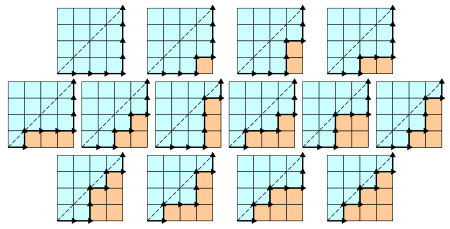
\includegraphics[height=100pt]{walk.png}
  \caption{$4 \times 4$ 网格的合法走法}
\end{figure}
\end{frame}

\begin{frame}[fragile]{卡特兰数}
以上几个问题都能得到一个相同的答案序列,这个序列即为卡特兰数。

卡特兰数可以由以下递推式得到:

$$
\begin{aligned}
C_{0} &= 1 \\
C_{n+1} &= \sum_{i=0}^{n} C_{i} C_{n-i} \quad (n \ge 0)
\end{aligned}
$$

数列的前几项为

$$
C = \{1, 1, 2, 5, 14, 42, 132, 429, 1430, 4862, 16796, ...\}
$$
\end{frame}

\begin{frame}[fragile]{卡特兰数:通项公式}

重新回到括号匹配的问题,我们将一个合法的括号序列记为 $c$,并将该括号序列的左右括号相互调换后的序列记为 $c'$。

显然对于所有的 $c$ 我们都可以唯一分解为 \verb|(| $c_1$ \verb|)| $c_2$ 的形式。

我们将任意一个左括号和右括号数量相等的序列记为 $b$,很显然有 $B_{n} = {2n \choose n}$。

考虑将 $b$ 拆解,发现我们可以将其唯一分解成 \verb|(| $c$ \verb|)| $b$ 或者 \verb|)| $c'$ \verb|(| $b$ 的形式。
\end{frame}

\begin{frame}[fragile]{卡特兰数:通项公式}
  \begin{columns}[T]
    \column{0.6\textwidth}
      为何能唯一分解成 \verb|(| $c$ \verb|)| $b$ 或 \verb|)| $c'$ \verb|(| $b$ 的形式?

      \vspace{2em}

      可以将括号重新想象成网格上的走法,我们只关心从原点离开之后第一次回到对角线的这一段路程。可以发现这段路程中除去第一步和最后一步之后也必定是一个合法的括号序列(或者是左右括号相反的合法序列),因此我们以第一次回到对角线的位置为分界线可以将 $b$ 拆解成上述的两个不同形式,并且拆解方案唯一。
    \column{0.4\textwidth}
      \begin{figure}
        \centering
        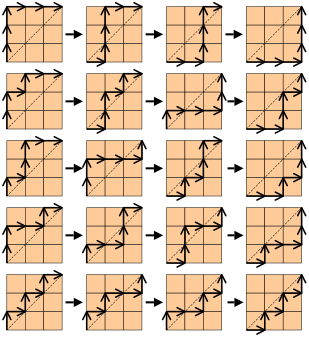
\includegraphics[height=150pt]{full_walk.png}
        \caption{$3 \times 3$ 网格的全部走法}
      \end{figure}
  \end{columns}
\end{frame}

\begin{frame}[fragile]{卡特兰数:通项公式}
  通过唯一分解的方法,我们可以得到以下公式

  $$
  B_{n+1} = 2 \sum_{i=0}^{n}B_{i}C_{n-i}
  $$

  考虑 $b$ 中不合法的情况,可以发现非法的括号序列必定以 $c$ \verb|)| 开头,因此有

  $$
  B_{n+1} - C_{n+1} = \sum_{i=0}^{n} {2i+1 \choose i} C_{n-i}
  $$
\end{frame}

\begin{frame}[fragile]{卡特兰数:通项公式}
  套用递归式可以得到

  $$
  \begin{aligned}
  B_{n+1} - C_{n+1} &= 2 \sum_{i=0}^{n} B_{i} C_{n-i} - \sum_{i=0}^n C_{i} C_{n-i} \\
  &= \sum_{i=0}^{n} (2 B_{i} - C_{i}) C_{n-i}
  \end{aligned}
  $$

  因此有

  $$
  2 B_{n} - C_{n} = {2n+1 \choose n}
  $$
\end{frame}

\begin{frame}[fragile]{卡特兰数:通项公式}
  化简得到

  $$
  \begin{aligned}
  C_{n} &= 2 B_{n} - {2n+1 \choose n} \\
  &= 2 {2n \choose n} - {2n+1 \choose n} \\
  &= \frac{1}{n+1} {2n \choose n}
  \end{aligned}
  $$

  这就是卡特兰数的通项公式
\end{frame}

\begin{frame}[fragile]{卡特兰数:通项公式}
  卡特兰数的其他公式

  $$
  \begin{aligned}
  C_{n} &= \frac{1}{n+1} {2n \choose n} \\
  &= {2n \choose n} - {2n \choose n - 1} \\
  &= \frac{4n-2}{n+1} C_{n-1}
  \end{aligned}
  $$
\end{frame}

\section[斯特林数]{Stirling Numbers}

\subsection[第二类斯特林数]{Stirling numbers of the second kind}

\begin{frame}[fragile]{第二类斯特林数}
第二类斯特林数 $\begin{Bmatrix}n\\ k\end{Bmatrix}$,也可记做 $S(n, k)$。

表示将 $n$ 个两两不同的元素,划分为 $k$ 个互不区分的非空子集的方案数。
\end{frame}

\begin{frame}[fragile]{第二类斯特林数:递推式}
我们插入一个新元素时,有两种方案

\begin{enumerate}
  \item 将新元素单独放入一个子集,有 $\begin{Bmatrix}n-1\\ k-1\end{Bmatrix}$ 种方案;
  \item 将新元素放入一个现有的非空子集,有 $k\begin{Bmatrix}n-1\\ k\end{Bmatrix}$ 种方案。
\end{enumerate}

$$
\begin{Bmatrix}n\\ k\end{Bmatrix} = \begin{Bmatrix}n-1\\ k-1\end{Bmatrix} + k\begin{Bmatrix}n-1\\ k\end{Bmatrix}
$$
\end{frame}

\begin{frame}[fragile]{第二类斯特林数:通项公式}
令 $g(k)$ 为将 $n$ 个元素分配到 $k$ 个不同的集合(允许空集)的方案数;

令 $f(k)$ 为将 $n$ 个元素分配到 $k$ 个不同的集合(不允许空集)的方案数。

显然我们有 $g(k) = k^n$,并且我们可以知道

$$
g(k) = \sum_{i=0}^{k} {k \choose i} f(i)
$$
\end{frame}

\begin{frame}[fragile]{第二类斯特林数:通项公式}
根据二项式反演,我们可以得到

$$
\begin{aligned}
f(k) &= \sum_{i=0}^{k} (-1)^{k-i} {k \choose i} g(i) \\
     &= \sum_{i=0}^{k} (-1)^{k-i} {k \choose i} i^n \\
     &= \sum_{i=0}^{k} \frac{(-1)^{k-i} i^n k!}{i! (k-i)!}
\end{aligned}
$$
\end{frame}

\begin{frame}[fragile]{第二类斯特林数:通项公式}
再考虑 $f(k)$ 与第二类斯特林数的关系,我们发现由于第二类斯特林数要求 $k$ 个集合之间互不区分,因此 $f(k)$ 相比于第二类斯特林数恰好多乘了一个 $k!$。

去掉 $f(k)$ 中的 $k!$ 项之后我们便可以得到第二类斯特林数的通项公式:

$$
\begin{Bmatrix}n\\ k\end{Bmatrix} = \sum_{i=0}^{k} \frac{(-1)^{k-i} i^n}{i! (k-i)!}
$$
\end{frame}

\begin{frame}[fragile]{例题:Add or Multiply 1}
  你有 $n$ 个不同的加法操作和 $m$ 个不同的乘法操作,求问能排列出多少种本质不同的计算式?

  例如以下两种方式得到的结果是相同的

  \begin{itemize}
    \item $(((x + a_1) + a_2) \times a_3)$
    \item $(((x + a_2) + a_1) \times a_3)$
  \end{itemize}

  $1 \le n, m \le 3000, 1 \le T \le 10^4$
\end{frame}

\begin{frame}[fragile]{例题:Add or Multiply 1}
  首先可以发现结果是若干个加法块和乘法块交替的排列。

  可以先枚举总共有多少个加法块和乘法块,再计算块中分配数字的方案数。

  如果当前枚举到有 $i$ 个加法块和 $j$ 个乘法块,那么就是求第二类斯特林数。

  $$
  f(i, j) = i! \times S(n, i) \times j! \times S(m, j) 
  $$

  这个函数可以 $O(n^2)$ 预处理,然后 $O(1)$ 求值。
\end{frame}

\begin{frame}[fragile]{例题:Add or Multiply 1}
  接着就是枚举加法块和乘法块的数量的问题了,我们可以直接枚举加法块的数量,然后乘法块的数量就只有可能是 $i-1, i, i+1$ 中的一种。

  当然对于 $j=i$ 的时候分为先乘后加和先加后乘两种方案,因此最终结果需要乘以二。

  $$
  \sum_{i=0}^{n} [f(i, i-1) + 2 \times f(i, i) + f(i, i+1)]
  $$

  单次求解的复杂度为 $O(n)$,总复杂度为 $O(n^2+Tn)$。
\end{frame}

\subsection[第一类斯特林数]{Stirling numbers of the first kind}

\begin{frame}[fragile]{第一类斯特林数}
第一类斯特林数 $\begin{bmatrix}n\\ k\end{bmatrix}$,也可记做 $s(n, k)$。

表示将 $n$ 个两两不同的元素,划分为 $k$ 个互不区分的非空轮换的方案数。

\begin{figure}
  \centering
  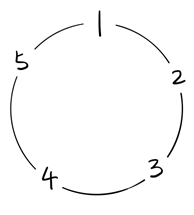
\includegraphics[height=100pt]{circle.png}
  \caption{轮换(圆排列)}
\end{figure}
\end{frame}

\begin{frame}[fragile]{第一类斯特林数:递推式}
我们插入一个新元素时,有两种方案

\begin{enumerate}
  \item 将新元素单独放入一个轮换,有 $\begin{bmatrix}n-1\\ k-1\end{bmatrix}$ 种方案;
  \item 将新元素放入一个现有的非空轮换,有 $(n-1)\begin{bmatrix}n-1\\ k\end{bmatrix}$ 种方案。
\end{enumerate}

$$
\begin{bmatrix}n\\ k\end{bmatrix} = \begin{bmatrix}n-1\\ k-1\end{bmatrix} + (n-1)\begin{bmatrix}n-1\\ k\end{bmatrix}
$$
\end{frame}

\begin{frame}[fragile]{第一类斯特林数:部分公式}
$$
\begin{aligned}
  s(0, 0) &= 1 \\
  s(n, 0) &= 0 \quad (n \ge 1) \\
  s(n, n) &= 1 \\
  s(n, 1) &= (n-1)! \\
  s(n, n-1) &= {n \choose 2} \\
  \sum_{k=0}^{n}s(n, k) &= n!
\end{aligned}
$$
\end{frame}

\begin{frame}[fragile]{例题:没有例题}
\begin{figure}
  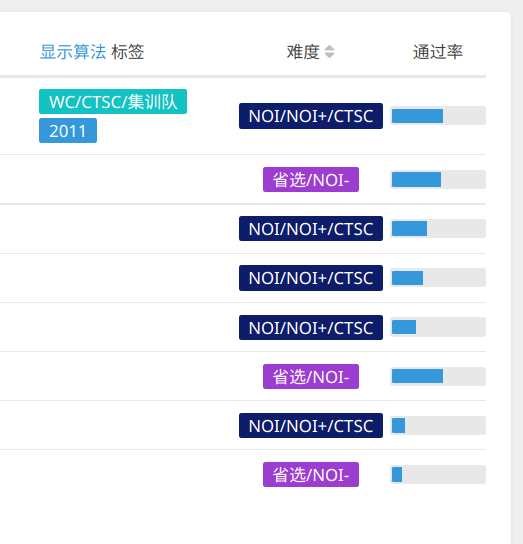
\includegraphics[height=200pt]{stirling.png}
\end{figure}
\end{frame}

\begin{frame}{}
  \centering \Large
  \emph{Good Luck \& Have Fun!}
\end{frame}

\end{document}